% !TEX root = ./0.main.tex

%In the industry, the sequential recommendation is a very demanding problem since, in e-commerce companies, we are facing users with long historical behaviors that rely on the predictions for recommendations. 
In this section, we experiment on the sequential recommendation to evaluate the performance of our framework compared with other state-of-the-art methods. Besides, we also report the experimental results of our framework on a billion-scale industrial dataset. 

\begin{table}
  \centering
  \caption{\label{tab:match_stats} Statistics of datasets.}
%   \renewcommand{\arraystretch}{1.2}
  \begin{tabular}{c|c|c|c}
    \hline \hline
    \textbf{Dataset} & \# users & \# items & \ \# interactions \\
    \hline
    Amazon Books & 459,133 & 313,966 & 8,898,041 \\
    % Amazon Electronics & 192,403 & 63001 & 1,689,188 \\
    % ML-20M & & & \\
    % Netflix & & & \\
    Taobao & 976,779 & 1,708,530 & 85,384,110 \\
    \hline \hline
  \end{tabular}
\end{table}

\begin{table*}[]
    \centering
    \caption{Model performance on public datasets. Bolded numbers are the best performance of each column. All the numbers in the table are percentage numbers with `\%' omitted.}
    % \renewcommand{\arraystretch}{1.2}
    \begin{tabular}{l|cccccc|cccccc}
        \hline \hline
        & \multicolumn{6}{c|}{Amazon Books} & \multicolumn{6}{c}{Taobao} \\
        & \multicolumn{3}{c}{Metrics@20} & \multicolumn{3}{c|}{Metrics@50} & \multicolumn{3}{c}{Metrics@20} & \multicolumn{3}{c}{Metrics@50} \\
        \hline
        & Recall & NDCG & Hit Rate & Recall & NDCG & Hit Rate & Recall & NDCG & Hit Rate & Recall & NDCG & Hit Rate \\
        \hline
        MostPopular & 1.368 & 2.259 & 3.020 & 2.400 & 3.936 & 5.226 & 0.395 & 2.065 & 5.424 & 0.735 & 3.603 & 9.309 \\
        YouTube DNN & 4.567 & 7.670 & 10.285 & 7.312 & 12.075 & 15.894 & 4.205 & 14.511 & 28.785 & 6.172 & 20.248 & 39.108 \\
        GRU4Rec & 4.057 & 6.803 & 8.945 & 6.501 & 10.369 & 13.666 & 5.884 & 22.095 & 35.745 & 8.494 & 29.396 & 46.068 \\
        % SASRec & & & & & & \\
        % Attention & 4.624 & 7.707 & 10.214 & 7.238 & 11.763 & 15.429 & & & & 2.496 & 29.808 & 47.845 \\
        MIND & 4.862 & 7.933 & 10.618 & 7.638 & 12.230 & 16.145 & 6.281 & 20.394 & 38.119 & 8.155 & 25.069 & 45.846 \\
        \hline
        \model-SA & \textbf{5.489} & 8.991 & 11.402 & \textbf{8.467} & \textbf{13.563} & 17.202 & \textbf{6.900} & \textbf{24.682} & 41.549 & 9.462 & 31.278 & 51.064 \\
        \model-DR & 5.311 & \textbf{9.185} & \textbf{12.005} & 8.106 & 13.520 & \textbf{17.583} & 6.890 & 24.007 & \textbf{41.746} & \textbf{9.818} & \textbf{31.365} & \textbf{52.418} \\
        \hline \hline
    \end{tabular}
    \label{tab:match_results}
\end{table*}

\subsection{Experimental Setup}

% The matching stage plays a crucial role in recommendations due to the large-scale item pool of industrial recommender systems. 

We evaluate the performance of all methods under strong generalization ~\cite{marlin2004collaborative, liang2018variational, ma2019learning}: We split all users into training/validation/test sets by the proportion of 8:1:1. We train models using the entire click sequences of training users. To evaluate, we take the first 80\% of the user behaviors from validation and test users to infer user embeddings from trained models and compute metrics by predicting the remaining 20\% user behaviors. This setting is more difficult than weak generalization where the users' behavior sequences are used during both training and evaluation processes~\cite{liang2018variational}.
In detail, we adopt a common setting of training sequential recommendation models. Let the behavior sequence of user $u$ be $(e_1^{(u)}, e_2^{(u)}, ..., e_k^{(u)}, ..., e_n^{(u)})$. Each training sample uses the first $k$ behaviors of $u$ to predict the $(k+1)$-th behavior, where $k=1,2,...,(n-1)$.

\vpara{Datasets.} We conduct experiments on two challenging public datasets. The statistics of the two datasets are shown in Table~\ref{tab:match_stats}. 

\begin{itemize}
    \item \textbf{Amazon}\footnote{\url{http://jmcauley.ucsd.edu/data/amazon/}} consists of product reviews and metadata from Amazon ~\cite{mcauley2015image,he2016ups}. In our experiment, we use the \textit{Books} category of the Amazon dataset. Each training sample is truncated at length 20.
    % \item \red{\textbf{MovieLens 20M}\footnote{https://grouplens.org/datasets/movielens/} consists of 20M movie ratings, which is a stable benchmark dataset. 20 million ratings and 465,000 tag applications are applied to 27,000 movies by 138,000 users. ML-20M includes tag genome data with 12 million relevance scores across 1,100 tags.}
    % \item \red{\textbf{Netflix}\footnote{http://www.netflixprize.com/} is user-movie rating data constructed to support participants in the Netflix Prize. The movie rating files contain over 100 million ratings from 480 thousand randomly-chosen, anonymous Netflix customers over 17 thousand movies. The data were collected between October, 1998 and December, 2005 and reflect the distribution of all ratings received during this period. The date of each rating and the title and year of release for each movie id are also provided.
    % }
    \item \textbf{Taobao}\footnote{\url{https://tianchi.aliyun.com/dataset/dataDetail?dataId=649\&userId=1}} collects user behaviors from Taobao's recommender systems~\cite{zhu2018learning}.  In our experiment, we only use the click behaviors and sort the behaviors from one user by time. Each training sample is truncated at length 50.
\end{itemize}
% For each user $u$, we sort the reviews from the user by time, and our task is to predict whether the user will write the review for the item based on previous reviews.
% Taobao dataset randomly selects about 1 million users who have behaviors including click, purchase, add-to-cart, and add-to-preference from November 25 to December 03, 2017. Each behavior is represented by five fields, which consist of user ID, item ID, item's category ID, behavior type, and timestamp.

\vpara{Competitors.} We compare our proposed models, \model-SA and \model-DR, with state-of-the-art models. In our experimental setting, models should give the prediction for the unseen users of validation and test sets. Thus factorization-based methods are inappropriate for this setting.
\begin{itemize}
    \item \textbf{MostPopular} is a traditional recommendation method that recommends the most popular items to users. 
    % \item \textbf{Embedding\&MLP} is a basic deep learning model for CTR prediction formalized by~\cite{zhou2018deep, zhou2019deep}. The input features of items are first mapped into low dimensional embedding vectors and then transformed into fixed-length vectors using a pooling operator. 
    \item \textbf{YouTube DNN}~\cite{covington2016deep} is one of the most successful deep learning models for industrial recommender systems.
    \item \textbf{GRU4Rec}~\cite{hidasi2015session} is the first work that introduces recurrent neural networks for the recommendation. 
    % It is worth mentioning that GRU4Rec can be used for either ranking task or matching task.
    % \item \textbf{ARNN} is a variation of GRU4Rec, which uses an attention mechanism to weighted sum over all the hidden states along time.
    % \item \textbf{RUM}~\cite{chen2018sequential} designs a memory-augmented neural network that integrated with the insights of collaborative filtering for the recommendation.
    % \item \textbf{SASRec}~\cite{kang2018self} captures long-term semantics by a self-attention based sequential model and makes predictions based on relatively few actions.
    \item \textbf{MIND}~\cite{li2019multi} is a recent state-of-the-art model related with our model. It designs a multi-interest extractor layer based on the capsule routing mechanism, which is applicable for clustering past behaviors and extracting diverse interests.
\end{itemize}

\vpara{Implementation Notes.}
The code used by our experiments is implemented with TensorFlow\footnote{\url{https://www.tensorflow.org/}} 1.14 in Python 3.6. % The experiments on the two datasets are conducted using a single Linux server with 4 Intel(R) Xeon(R) CPU E5-2680 v4 @ 2.40GHz, 256G RAM, and 8 NVIDIA GeForce RTX 2080 Ti.
% The experiment is conducted using dozens of workers of Alibaba distributed cloud platform\footnote{https://data.aliyun.com/}. Every two workers share an NVIDIA Tesla P100 GPU with 16GB memory.

\vpara{Parameter Configuration.}
The number of dimensions $d$ for embeddings is set to 64. The number of samples for sampled softmax loss is set to 10. The number of maximum training iterations is set to 1 million. The number of interest embeddings for multi-interest models is set to 4. We use Adam optimizer~\cite{kingma2014adam} with learning rate $lr=0.001$ for optimization.

% The batch size for the Amazon dataset and Taobao dataset is set to 128 and 256, respectively. The number of iterations for the dynamic routing method is set to 3.

\vpara{Evaluation Metrics.}
We use the following metrics to evaluate the performance of our proposed model. We use three commonly used evaluation criteria in our experiments. 
\begin{itemize}
    \item \textbf{Recall}. We adopt per-user average instead of global average for better interpretability~\cite{karypis2001evaluation,chen2018sequential}.
        \begin{equation}
            \operatorname{Recall@N} = \frac{1}{|\mathcal{U}|}\sum_{u\in \mathcal{U}} \frac{|\mathcal{\hat{I}}_{u,N} \cap \mathcal{I}_{u}|}{|\mathcal{I}_u|},
        \end{equation}
        where $\mathcal{\hat{I}}_{u,N}$ denotes the set of top-N recommended items for user $u$ and $\mathcal{I}_u$ is the set of testing items for user $u$.
    
    \item \textbf{Hit Rate}. Hit rate (HR) measures the percentage that recommended items contain at least one correct item interacted by the user, which has been widely used in previous works~\cite{karypis2001evaluation,chen2018sequential}.
        \begin{equation}
            \operatorname{HR@N} = \frac{1}{|\mathcal{U}|}\sum_{u\in \mathcal{U}} \delta(|\mathcal{\hat{I}}_{u,N} \cap \mathcal{I}_{u}|>0),
        \end{equation}
        where $\delta(\cdot)$ is the indicator function.
        % where $\mathcal{\hat{I}}_{u,N}$ denotes the set of top-$N$ recommendation items for user $u$ and $\mathcal{I}_u^{+}$ is the set of positive testing items for user $u$. $\delta(\cdot)$ is the indicator function.

    % \item \textbf{Mean Average Precision (MAP)}. There is only one target item per instance and thus the MAP@N increases with N which is consistent with ~\cite{belletti2018factorized,tang2019towards}.
    %     \begin{equation}
    %         \operatorname{MAP@N} = \frac{1}{|\mathcal{U}|}\sum_{u\in \mathcal{U}}  \frac{\sum_{k=1}^N P_u@k\times \delta(\hat{i}_{u,k}\in \mathcal{I}_u^{+})}{|\mathcal{\hat{I}}_{u,N}\cap \mathcal{I}_u^{+}|},
    %     \end{equation}
    %     \begin{equation}
    %         P_u@k = \frac{|\mathcal{\hat{I}}_{u,k}\cap \mathcal{I}_u^{+}|}{|\mathcal{\hat{I}}_{u,k}|},
    %     \end{equation}
    %     where $\mathcal{\hat{I}}_{u,N}$ denotes the set of top-$N$ recommendation items for user $u$, $\mathcal{I}_u^{+}$ is the set of positive testing items for user $u$, $\hat{i}_{u,k}$ denotes the $k$-th recommendation item, and $\delta(\cdot)$ denotes the indicator function. 


    \item \textbf{Normalized Discounted Cumulative Gain}. Normalized Discounted Cumulative Gain (NDCG) takes the positions of correct recommended items into consideration~\cite{jarvelin2000ir}.
        \begin{equation}
            \operatorname{NDCG@N} = \frac{1}{Z}\operatorname{DCG@N} = \frac{1}{Z} \frac{1}{|\mathcal{U}|}\sum_{u\in\mathcal{U}}\sum_{k=1}^{N}\frac{\delta(\hat{i}_{u,k}\in \mathcal{I}_{u})}{\operatorname{log}_2(k+1)},
        \end{equation}
        where $\hat{i}_{u,k}$ denotes the $k$-th recommended item for the user $u$, and $Z$ is a normalization constant denoting the ideal discounted cumulative gain (IDCG@N), which is the maximum possible value of DCG@N. 
\end{itemize}

% \begin{figure*}
%     \centering
%     \includegraphics[width=0.9\textwidth]{figures/heatmap.pdf}
%     \caption{The heatmap of a user's four interests and the behavior sequence from the Amazon dataset. From the heatmap, we can see that our model learns four different interests from the behavior sequence. The 0th, 1st, 2nd, and 3rd interests are related to the ``Health'', ``Business'', ``Cookbooks'', and ``Self-Help'' categories, respectively. Our model learns the category information from the user sequence, although only item IDs are used for model training.}
%     \label{fig:case_study_heatmap}
% \end{figure*}


% \begin{table*}[]
%     \centering
%     \caption{Book titles and categories of the user behavior sequence from the Amazon dataset.}
%     \begin{tabular}{c|l|l}
%         \hline \hline
%         No. & Book Title & Category \\
%         \hline
%         0 & MAKE MONEY ONLINE ON ELANCE & Business \& Money \\
%         1 & Cure Acne Overnight & Health, Fitness \& Dieting \\
%         2 & Headling Your Inner Child & Self-Help \\
%         3 & SOCIAL MEDIA MARKETING FOR BEGINNERS & Business \& Money \\
%         4 & POSITIVE THINKING: The Ultimate Guide To Mastering Positive Thinking & Self-Help \\
%         5 & COMMUNICATION SKILLS Secrets & Self-Help \\
%         6 & THE MEDITERRANEAN DIET ROCKS!!! & Cookbooks, Food \& Wine \\
%         7 & REAL ESTATE WHOLESALING REVEALED & Business \& Money \\
%         8 & HOW TO GET CUSTOMERS IN YOUR NETWORK MARKETING COMPANY & Business \& Money \\
%         9 & THE PALEO COMFORT FOODS COOKBOOK & Cookbooks, Food \& Wine \\
%         10 & CREATIVITY: Discover How To Unlock Your Creative Genius And Release The Power Within & Health, Fitness \& Dieting \\
%         11 & GREEK CUISINE COOKBOOK & Cookbooks, Food \& Wine \\
%         12 & Gluten-Free Vegan Cookbook & Cookbooks, Food \& Wine \\
%         \hline \hline
%     \end{tabular}
%     \label{tab:case_study_cate}
% \end{table*}

\subsection{Quantitative Results}
% \subsection{Performance Analysis.}
To make a fair comparison with other models, we set $\lambda=0$ in our aggregation module. We give a detailed illustration of retrieving top-N items of our framework. For our framework, each interest of a user independently retrieves top-N candidate items. Thus, our model retrieves a total of $K\cdot N$ items for each user. We sort the items by the inner product of the item embedding and the corresponding interest embedding. After the sorting, top-N items from these $K\cdot N$ items are viewed as the final candidate items of our model. The way of retrieving candidate items is also applied to MIND. 
The model performance for the sequential recommendation is shown in Table~\ref{tab:match_results}. Our models outperform all state-of-the-art models by a wide margin on all the evaluation criteria. GRU4Rec obtains the best performance over other models that only output single embedding for each user. Compared with MIND, \model-DR obtains better performance due to the difference of the dynamic routing method. \model-SA shows the strong ability to capture user interests by the self-attention mechanism and gets comparable results with \model-DR.
% The performance shows that our model has a strong ability to capture user interests. 
%With the penalty term, multiple interests of users can be better disentangled and the performance improves. 


% \begin{figure}[t]
%     \centering
% %     \subfigure[Interest Number]{\includegraphics[width=0.23\textwidth]{figures/interest_num.png}}
% %  	\subfigure[Iteration Number]{\includegraphics[width=0.23\textwidth]{figures/iteration_num.png}}
%     \includegraphics[width=0.50\textwidth]{figures/sensitivity.pdf}
% 	\caption{Model performance w.r.t. the number of user interests and the iteration of the dynamic routing method}
%     \label{fig:ctr_sensitivity}
% \end{figure}

\begin{table}
  \centering
  \caption{\label{tab:match_ps} Model performance of parameter sensitivity. All the numbers are percentage numbers with `\%' omitted.}
%   \renewcommand{\arraystretch}{1.2}
  \begin{tabular}{l|cc|cc}
    \hline \hline
    & \multicolumn{2}{c|}{Amazon Books} & \multicolumn{2}{c}{Taobao} \\
    Metric@50 & Recall & NDCG & Recall & NDCG \\
    \hline
    \model-SA (K=2) & 8.835 & \textbf{14.273} & 9.935 & 32.873 \\
    \model-SA (K=4) & 8.467 & 13.563 & 9.462 & 31.278 \\
    \model-SA (K=6) & \textbf{8.901} & 14.167 & 9.378 & 31.020 \\
    \model-SA (K=8) & 8.547 & 13.631 & 9.493 & 31.196 \\
    \hline
    \model-DR (K=2) & 7.081 & 12.068 & 9.293 & 30.735 \\
    \model-DR (K=4) & 8.106 & 13.520 & 9.818 & 31.365 \\
    \model-DR (K=6) & 7.904 & 13.219 & 10.836 & \textbf{34.048} \\
    \model-DR (K=8) & 7.760 & 12.900 & \textbf{10.841} & 33.895 \\
    \hline \hline
  \end{tabular}
\end{table}

\vpara{Parameter Sensitivity.}
We investigate the sensitivity of the number of interests $K$ of our framework. Table~\ref{tab:match_ps} illustrates the performance of our framework when the hyperparameter $K$ changes. Our two models show the different properties of this hyperparameter. For the Amazon dataset, \model-SA obtains the better performance when $K=2, 6$ and \model-DR gets the best result when $K=4$. For the Taobao dataset, \model-DR gets better performance when $K$ increases from 2 to 8 but \model-SA obtains the best result when $K=2$.

\begin{table}
  \centering
  \caption{\label{tab:control} Model performance of Amazon dataset for the controllable study. All the numbers are percentage numbers with `\%' omitted.}
%   \renewcommand{\arraystretch}{1.2}
  \begin{tabular}{c|cc|cc}
    \hline \hline
    & \multicolumn{2}{c|}{\model-SA (K=4)} & \multicolumn{2}{c}{\model-DR (K=4)} \\
    Metric@50 & Recall & Diversity & Recall & Diversity \\
    \hline
    $\lambda=0.00$ & \textbf{8.467} & 23.237 & \textbf{8.106} & 19.036 \\
    $\lambda=0.05$ & 8.347 & 38.808 & 7.931 & 42.915 \\
    $\lambda=0.10$ & 8.229 & 46.731 & 7.850 & 46.258 \\
    $\lambda=0.15$ & 8.142 & 51.135 & 7.820 & 46.912 \\
    $\lambda=0.20$ & 8.086 & 53.671 & 7.783 & 47.581 \\
    $\lambda=0.25$ & 8.034 & \textbf{55.100} & 7.764 & \textbf{48.375} \\
    \hline \hline
  \end{tabular}
\end{table}

\subsection{Controllable Study}
\label{sec:control_study}
% Our proposed model generates multiple embeddings for each user. 
%A straightforward method is to sort the items based on their scores. However, each interest of a user is not equally important.
To obtain the final top-N candidate items for each user, we propose a novel module to aggregate the items retrieved by different interests of each user. 
In addition to aim at achieving high prediction accuracy for the recommendation, some studies suggest the need for diversified recommendations to avoid monotony and improve customers' experience~\cite{gogna2017balancing,cheng2017learning}. 

Recommendation diversity plays a more important role in current recommender systems. Many pieces of research target on improving the recommendation diversity~\cite{bradley2001improving,qin2013promoting}. Our proposed aggregation module can control the balance of recommendation accuracy and diversity. We use the following definition of individual diversity based on item categories:
\begin{equation}
    \operatorname{Diversity@N} = \frac{\sum_{j=1}^N \sum_{k=j+1}^N \delta(\operatorname{CATE}(\hat{i}_{u,j}) \neq \operatorname{CATE}(\hat{i}_{u,k}))}{N \times (N-1) / 2},
\end{equation}
\noindent where $\operatorname{CATE}(i)$ is the category of item $i$, $\hat{i}_{u,j}$ denotes the $j$-th recommended item for the user $u$, and $\delta(\cdot)$ is an indicator function. 

Table~\ref{tab:control} shows the model performance of the Amazon dataset when we control the factor $\lambda$ to balance the recommendation quality and diversity. From the table, recommendation diversity increases substantially and recall decreases slightly when the controllable factor $\lambda$ increases. Our aggregation module can achieve the optimum trade-off between the accuracy and diversity by choosing an appropriate value for the hyperparameter $\lambda$.


% \vpara{Ablation Study.}


% \begin{itemize}
%     \item \textbf{Precision, Recall, and F1-score}. We adopt the global average of all the users as follows. 
%         \begin{equation}
%             \operatorname{Precision} = \frac{\sum_{u\in \mathcal{U}}\sum_{i\in \mathcal{I}_u^{+}}\delta(\hat{y}_{ui}=1)}{\sum_{u\in \mathcal{U}}\sum_{i\in \mathcal{I}_u^{+} \cup \mathcal{I}_u^{-}}\delta(\hat{y}_{ui}=1)},
%         \end{equation}
%         \begin{equation}
%             \operatorname{Recall} = \frac{\sum_{u\in \mathcal{U}}\sum_{i\in \mathcal{I}_u^{+}}\delta(\hat{y}_{ui}=1)}{\sum_{u\in \mathcal{U}}|\mathcal{I}_u^{+}|},
%         \end{equation}
%         \begin{equation}
%             \operatorname{F1} = \frac{2\cdot \operatorname{Precision} \cdot \operatorname{Recall}}{\operatorname{Precision} + \operatorname{Recall}},
%         \end{equation}
%         where $\mathcal{I}_u^{+/-}$ is the set of positive/negative testing items, $\hat{y}_{ui}$ is the prediction of user $u$ interacting with item $i$, and $\delta(\cdot)$ is the indicator function. 
%     \item \textbf{AUC}. AUC is one of the most important evaluation metrics for measuring the performance of classification model.
%         \begin{equation}
%         \operatorname{AUC} =  \frac{1}{|\mathcal{D}^{+}||\mathcal{D}^{-}|} \sum_{(u,j)\in \mathcal{D}^{+}} \sum_{(v,k)\in \mathcal{D}^{-}} \delta(\hat{p}_{u,j} > \hat{p}_{v,k}),
%         \end{equation}
%         where $\mathcal{D}^{+/-}$ is the set of positive/negative training samples, $\hat{p}_{u,j}$ is the predicted probability, and $\delta(\cdot)$ is the indicator function. 
% \end{itemize}


% \vpara{Performance Analysis.}
% The experimental results for the ranking task are shown in Table~\ref{tab:rank_results}. The mean with the standard error of AUC and F1-score is reported. All figures are trained for 10 times with random seed from 1 to 10. For the Amazon dataset, our model performs as well as MIMN and surpasses other models significantly. Our model takes much less time than MIMN for training as MIMN uses complicated architecture based on memory networks. For the Taobao dataset, our model outperforms all state-of-the-art models by a wide margin. The performance shows that our model has a strong ability to capture long-term and short-term user interests. % With the penalty term, multiple interests of users can be better disentangled and the performance improves on Taobao dataset. 


% \vpara{Ablation Study.}
% To show how each encoder contributes to the overall performance, we present the ablation study on our ranking model. We use T, S, L to denote the tiny-term, short-term, and long-term encoders, respectively. Our multi-interest capsule network can be viewed as a long-term encoder. We report the performance of our model using a different configuration of encoders as Table~\ref{tab:ctr_ablation} shows. In the Amazon dataset, our long-term encoder is a crucial part of the overall model. In the Taobao dataset, the combination of the tiny-term and short-term encoders obtains the best performance. The result shows that different encoders play different roles in the ranking task on different datasets. The difference between the two datasets may be caused by different types of behaviors. The Amazon dataset collects user review sequences, and the Taobao dataset collects user click sequences. The click behaviors rely more on tiny-term and short-term behaviors than review behaviors. From the ablation study, we can also see that mixture models obtain better performance than the single model. It is consistent with our motivation that a single model has limitations, and a mixture model is needed for the ranking stage of recommender systems. 


\subsection{Industrial Results}

\begin{table}
  \centering
  \caption{\label{tab:industrial_stats} Statistics of the industrial dataset}
%   \renewcommand{\arraystretch}{1.2}
  \begin{tabular}{c|c|c|c}
    \hline \hline
    \textbf{Dataset} & \# users & \# items & \# interactions \\
    \hline
    Industrial & 145,606,322 & 22,554,170 & 4,322,505,616 \\
    \hline \hline
  \end{tabular}
\end{table}


% \begin{figure}
%     \centering
%     \includegraphics[width=0.48\textwidth]{figures/tmp_picture.pdf}
%     \caption{The architecture of Taobao's recommender system.}
%     \label{fig:taobao_rs}
% \end{figure}

% The architecture of Taobao's recommender system is described as Figure~\ref{fig:taobao_rs}.

We further experiment on the industrial dataset collected by Mobile Taobao App on February 8th, 2020. The statistics of the industrial dataset are shown in the Table~\ref{tab:industrial_stats}. The industrial dataset contains 22 million high-quality items, 145 million users, and 4 billion behaviors between them. %\footnote{https://data.aliyun.com/}

Our framework has been deployed on the Alibaba distributed cloud platform, where every two workers share an NVIDIA Tesla P100 GPU with 16GB memory. We split the users and use the click sequences of training users to train our model. To evaluate, we use our model to compute multiple interests for each user in the test set. Each interest vector of a user independently retrieves top-N items from the large-scale item pool by a fast nearest neighbor method. The items retrieved by different user interests are fed into our aggregation module. After this module, top-N items out of $K\cdot N$ items are the final candidate items and are used to compute the evaluation metric, recall@50. 

We conduct an offline experiment between our framework and the state-of-the-art sequential recommendation method, MIND~\cite{li2019multi}, which has shown significant improvement in the recommender system of Alibaba Group. The experimental result demonstrates that our \model-SA and \model-DR improve recall@50 by 1.39\% and 8.65\% compared with MIND, respectively.

\begin{figure}
    \centering
    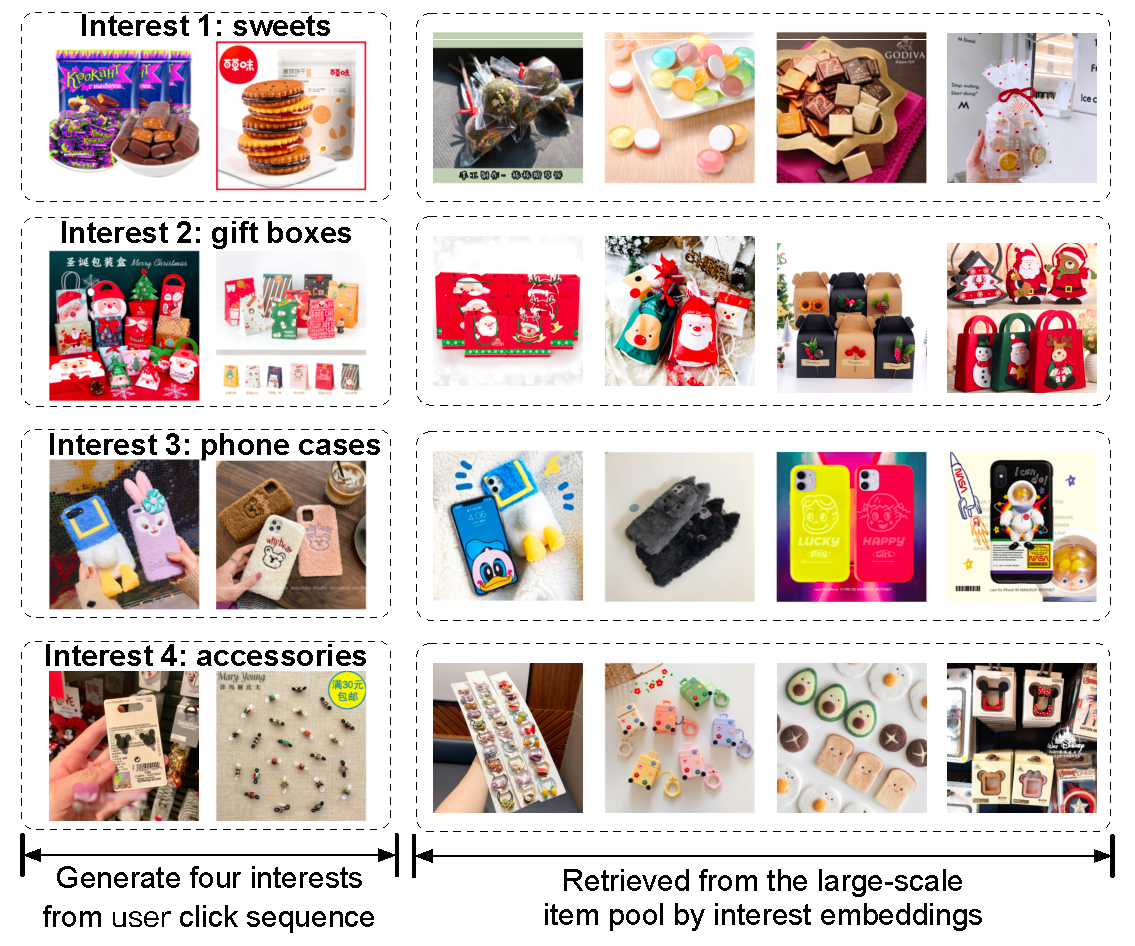
\includegraphics[width=0.47\textwidth]{figures/case_study.pdf}
    \caption{A case study of an e-commerce user. We generate four interest embeddings from the click sequence of a user by our model. We find that the four interests of the user are about sweets, gift boxes, phone cases, and accessories. We report those items in the click sequence that correspond to the four interests. The right part shows the items retrieved from the industrial item pool by interest embeddings. }
    \label{fig:case_study_interests}
\end{figure}


\vpara{Case Study.}
From the Figure~\ref{fig:case_study_interests}, we can see that our model learns four different interests of the user from her click sequence. It is worth noting that our model only uses item IDs for training and does not use the manually defined category information of items. Despite that, our model still can learn the item categories from user behavior sequences. Each interest learned by our model approximately corresponds to one specific category and can retrieve similar items of the same category from the large-scale industrial item pool. 


% The experimental goal is to maximize hit rate@N. We conduct an offline test on our matching model and xx. The results demonstrate that our model improves the hit rate by xx\% compared to xx.
